\documentclass[11pt,a4paper]{article}
\usepackage[utf8]{inputenc}
\usepackage[T1]{fontenc}
\usepackage{amsmath,amssymb,amsfonts}
\usepackage{graphicx}
\usepackage{hyperref}
\usepackage{booktabs}
\usepackage{geometry}
\usepackage{xcolor}
\usepackage{tikz}
\usepackage{pgfplots}
\pgfplotsset{compat=1.18}

\geometry{margin=2.5cm}

\hypersetup{
    colorlinks=true,
    linkcolor=blue,
    citecolor=blue,
    urlcolor=blue
}

\title{\textbf{R(k,S) as a Regime Response Surface in Energy-Flow Cosmology}\\[0.5em]
\large A Unified Framework for Structure-Dependent Gravitational Response}

\author{Morten Magnusson\\
\small ORCID: \href{https://orcid.org/0009-0002-4860-5095}{0009-0002-4860-5095}\\[0.5em]
\small DOI: \href{https://doi.org/10.6084/m9.figshare.31211437}{10.6084/m9.figshare.31211437}}

\date{January 2026}

\begin{document}

\maketitle

\begin{center}
\fbox{\parbox{0.9\textwidth}{
\textbf{Scope}: This is a theoretical framework paper. It introduces a coordinate system for gravitational response, derives testable structure, and specifies falsification criteria. It does not perform quantitative fits, MCMC analysis, or Boltzmann-code implementation. Those are subsequent steps that this framework enables.
}}
\end{center}

\begin{abstract}
We extend Energy-Flow Cosmology (EFC) phenomenology from time-dependent modified gravity parameters $\mu(a)$ and $\mu(k,z)$ to a state-dependent response surface $R(k,S)$, where $S$ is a derived, model-dependent state variable quantifying nonlinear structure accumulation. This synthesizes two prior results: the regime-dependent transition estimator (Fugaku--DESI) and the operational $\mu(k,z)$ formalism (weak lensing phenomenology). We derive falsification criteria against DES Y6 data. The core prediction: the L1$\to$L2 transition (CMB to late-universe) explains the $S_8$ tension, not probe-dependent variation within L2. This paper presents theoretical infrastructure for testing, not claimed validation.
\end{abstract}

\vspace{1em}
\noindent\fbox{\parbox{\textwidth}{
\textbf{Core Postulate:} The gravitational response $\mu$ in late-universe structure formation depends on the accumulated structural state $S$, not merely on cosmic time.

\medskip
Formally: $\mu = \mu(k, S)$ where $S = S(z)$ is a derived measure of nonlinear maturity.

\medskip
This implies: (1) $\mu \approx 1$ when $S \approx 0$ (linear regime, CMB epoch), and (2) $\mu \neq 1$ when $S > 0$ (nonlinear regime, late universe).

\medskip
The framework is falsifiable: a single $R(k,S)$ surface must describe all late-universe probes consistently.
}}

\vspace{1em}
\noindent\fbox{\parbox{\textwidth}{
\textbf{Regime Coordinate Principle:} \textit{Different cosmological probes do not measure different physics---they sample different coordinates $(k, S)$ on a single gravitational response surface.}
}}

\section{Introduction: What Are We Modeling?}

Cosmological observations present a consistent pattern:

\begin{table}[h]
\centering
\begin{tabular}{lll}
\toprule
\textbf{Regime} & \textbf{Observation} & \textbf{Gravitational behavior} \\
\midrule
L1 (CMB, $z\sim1100$) & Planck temperature + polarization & $G_\mathrm{eff} \approx G$ (standard GR) \\
L2 (Late universe, $z<2$) & Weak lensing, RSD, cluster counts & $G_\mathrm{eff} > G$ (enhanced growth) \\
\bottomrule
\end{tabular}
\end{table}

The $S_8$ tension---where late-universe probes consistently measure $S_8 \approx 0.78$--$0.79$ while CMB implies $S_8 \approx 0.83$---can be interpreted as evidence that \textbf{gravitational response depends on structural state}.

This interpretation does not require new gravity everywhere. It requires a \textbf{response function} that activates when the universe transitions from linear to nonlinear structure formation.

Two prior EFC papers establish the foundation:

\begin{enumerate}
    \item \textbf{Fugaku--DESI Transition Metric} \cite{fugaku}: Demonstrates that a single $\mu(a)$ function satisfying $\mu\approx1$ at recombination and $\mu>1$ at late times can reinterpret apparent matter density offsets as regime-dependent gravitational coupling.
    
    \item \textbf{EFC Weak Lensing Phenomenology} \cite{weaklens}: Introduces an operational closure (Postulate A) yielding $\mu(k,z)$ in standard cosmological perturbation form, enabling direct comparison with survey data.
\end{enumerate}

The present work extends these results by replacing \textbf{cosmic time ($z$)} with \textbf{structural state ($S$)} as the fundamental variable controlling gravitational response.

\section{Existing EFC Foundation}

\subsection{$\mu(a)$: Regime-Dependent Coupling (Fugaku--DESI)}

The Fugaku--DESI analysis defines a transition estimator:
\begin{equation}
\Delta_F \equiv \int W(a)\,[\mu(a)-1]\,d\ln a
\end{equation}
where $W(a)$ represents the observational sensitivity window. Key results:
\begin{itemize}
    \item $\mu \approx 1$ at recombination: Preserves CMB constraints
    \item $\mu > 1$ at late times: Consistent with enhanced structure growth
    \item $\Delta_F \approx 0.1$: Empirical constraint on integrated transition strength
\end{itemize}

This establishes that \textbf{one transition function can connect multiple regimes}.

\subsection{$\mu(k,z)$: Operational Field Closure (Weak Lensing)}

The weak lensing phenomenology paper derives:
\begin{equation}
k^2 \Phi = -4\pi G a^2 \mu(k,z)\,\bar{\rho}\,\delta
\end{equation}
where $\mu(k,z)$ emerges from Postulate A coupling entropy production to matter density. This places EFC in \textbf{standard cosmological perturbation formalism}.

\section{$S$ as a Structural State Variable}

\subsection{Physical Motivation}

Cosmic time $z$ is a \textbf{proxy} for what physically matters: the degree of nonlinear structure accumulation. We therefore define a structural maturity parameter:
\begin{equation}
S(z) \equiv \ln\left[\frac{\sigma^2(R_8, z)}{\sigma^2_{\mathrm{lin}}(R_8, z)}\right]
\end{equation}
where $R_8 = 8\,h^{-1}$Mpc is the standard smoothing scale and $\sigma^2_{\mathrm{lin}}$ is the linear-theory prediction.

\subsection{Operational Definition}

For practical implementation:
\begin{equation}
S(z) = \ln\left[\frac{\sigma_8^2(z)}{\sigma_{8,\mathrm{lin}}^2(z)}\right] = \ln\left[\frac{D^2(z) \cdot \sigma_8^2(z=0)}{D^2_{\mathrm{lin}}(z) \cdot \sigma_{8,\mathrm{lin}}^2(z=0)}\right]
\end{equation}

This is deterministic given a background cosmology---\textbf{$S$ is not a free parameter per data point}.

\subsection{Regime Interpretation}

\begin{table}[h]
\centering
\begin{tabular}{lll}
\toprule
\textbf{Regime} & \textbf{$S$ value} & \textbf{Physical meaning} \\
\midrule
L1 (CMB) & $S \approx 0$ & Linear universe, $\sigma \approx \sigma_{\mathrm{lin}}$ \\
L1$\to$L2 transition & $0 < S < 1$ & Nonlinear growth initiating \\
Late L2 & $S > 1$ & Structure-dominated dynamics \\
\bottomrule
\end{tabular}
\end{table}

This makes the model \textbf{regime-based} (EFC-consistent), \textbf{operationally defined} (computable under a specified nonlinear mapping), and \textbf{physically grounded} (measures accumulated nonlinearity).

\textbf{Important caveat}: $S$ depends on the choice of smoothing scale ($R_8$), nonlinear model (halofit, emulator, or N-body calibration), and reference linear prediction. It is therefore a \textit{derived} state variable, not a direct observable.

\textbf{Robustness}: Different nonlinear prescriptions yield monotonic transformations of $S$, preserving regime ordering even when the exact numerical scale varies. The physically meaningful content is the \textit{ordering} of states ($S_1 < S_2$ implies less nonlinear structure), not the absolute value.

\section{The $R(k,S)$ Response Surface}

\subsection{Definition}

We generalize the modified gravity parameter to:
\begin{equation}
\mu(k,S) = 1 + R(k,S)
\end{equation}
where $R(k,S)$ is the \textbf{regime response function} encoding how gravitational coupling deviates from GR as a function of both scale $k$ and structural state $S$.

\textbf{Critical constraint}: $R(k,S)$ is not a free function per probe; it is a single global surface that must simultaneously describe all late-universe observables. This is what makes the framework falsifiable.

\subsection{Minimal Parametrization}

A first-order Taylor expansion around a reference point $(k_0, S_0)$:
\begin{equation}
R(k,S) = R_0 \left[1 + a\ln\left(\frac{k}{k_0}\right) + b(S-S_0) + c\ln\left(\frac{k}{k_0}\right)(S-S_0)\right]
\end{equation}

This expansion is phenomenological and valid only locally in $(k,S)$-space.

\textbf{Parameters}:
\begin{itemize}
    \item $R_0$: Overall response amplitude
    \item $a$: Scale dependence (positive = stronger response at small scales)
    \item $b$: State dependence (positive = stronger response at higher $S$)
    \item $c$: Scale--state interaction
\end{itemize}

\textbf{Limiting case}: Setting $c = 0$ reduces the model to separable scale and state dependence, providing a controlled null hypothesis.

\textbf{Theoretical justification}: Locally, any smooth response surface can be expanded to first order; this represents the most general phenomenological form near a reference regime point. The logarithmic scale dependence $\ln(k/k_0)$ is standard in modified gravity phenomenology.

\textbf{Reference point choice}: $(k_0, S_0)$ should be chosen where data are most constraining---typically $k_0 \sim 0.1\,h/$Mpc and $S_0$ corresponding to $z \sim 0.5$. This is a coordinate choice, not an additional free parameter.

\subsection{Effect on Structure Growth}

In linear perturbation theory, $\mu > 1$ enhances the gravitational source term, modifying the growth equation. To first order, positive $R(k,S)$ leads to \textit{enhanced} gravitational response relative to GR, with magnitude depending on the integrated response history.

\textbf{Note}: The precise mapping from $R(k,S)$ to observable quantities ($S_8$, $f\sigma_8$, etc.) requires solving the modified perturbation equations. The relation is not a simple multiplicative correction.

\section{DES Y6 Consistency and the L1$\leftrightarrow$L2 Test}

\subsection{Key Observational Fact}

Recent DES Year 6 analyses report:
\begin{itemize}
    \item 3$\times$2pt $S_8 \approx 0.79$ (with uncertainty $\sim$0.01)
    \item CMB (Planck+ACT+SPT) $S_8 \sim 0.83$
    \item Tension: $\sim$2$\sigma$ in full parameter space
\end{itemize}

Critically, DES Y6 shows \textbf{good internal consistency} between cosmic shear, galaxy clustering, and galaxy-galaxy lensing. The tension is not between L2 probes---it is between L1 (CMB) and L2 (late universe).

\subsection{Model Prediction}

\begin{table}[h]
\centering
\begin{tabular}{llll}
\toprule
\textbf{Epoch} & \textbf{$S$ value} & \textbf{$R(k,S)$} & \textbf{Observed $S_8$} \\
\midrule
CMB ($z\sim1100$) & $S \approx 0$ & $R \approx 0$ & $\sim$0.83 (Planck) \\
DES ($z\sim0.3$--1.0) & $S > 0$ & $R > 0$ & $\sim$0.79 (suppressed) \\
\bottomrule
\end{tabular}
\end{table}

The sign of $R$ determines whether inferred $S_8$ is enhanced or suppressed relative to the $\Lambda$CDM baseline. In this framework, $R > 0$ (enhanced $\mu$) leads to \textit{lower} inferred $S_8$ from late-universe probes. The physical intuition: a stronger effective gravitational coupling allows observed clustering to arise from a lower primordial fluctuation amplitude---gravity does more work, so less initial ``seed'' is needed.

The \textbf{gradient in $S$} explains the L1$\to$L2 offset without requiring different physics for different L2 probes.

\subsection{Why L2 Probes Are Internally Consistent}

Different late-universe probes (WL, RSD, clusters) sample different $(k, S)$ windows on the same response surface. If the $c$ coefficient (k$\times$S interaction) is small, they see similar $R$ values. This explains:
\begin{itemize}
    \item WL and galaxy clustering agreeing within L2
    \item Both disagreeing with CMB (different $S$ regime)
\end{itemize}

\section{Visualization: The $R(k,S)$ Response Surface}

Figure~\ref{fig:response} illustrates the regime response surface and probe coverage.

\begin{figure}[htbp]
\centering
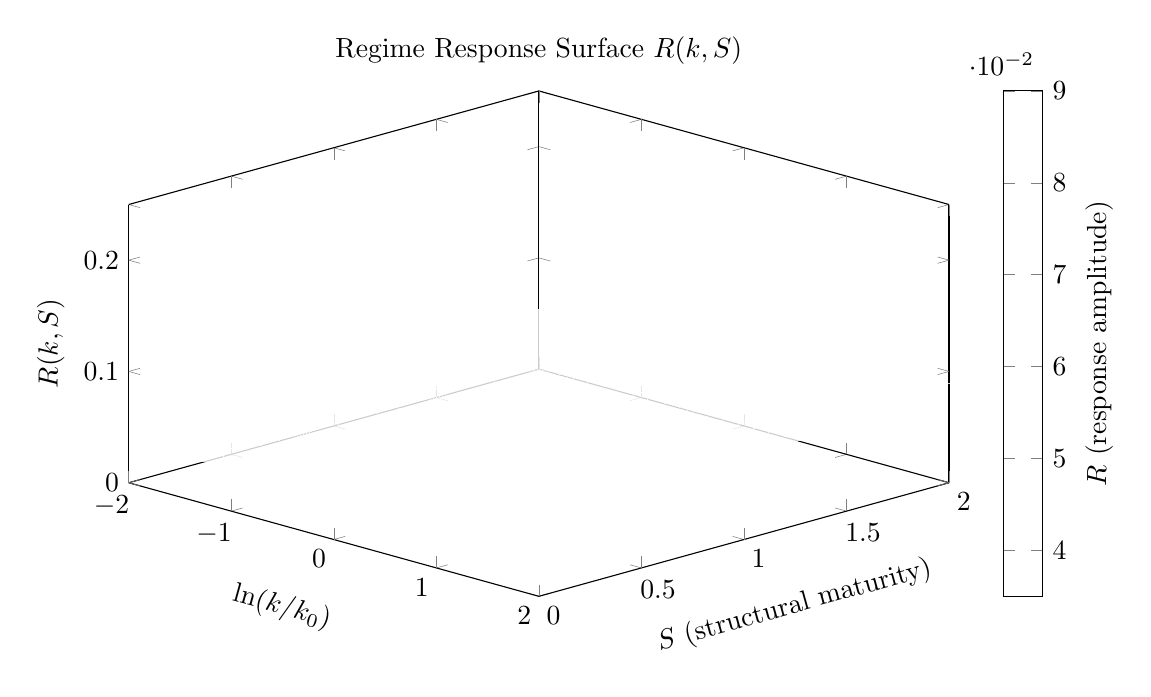
\begin{tikzpicture}
\begin{axis}[
    width=12cm,
    height=8cm,
    xlabel={$\ln(k/k_0)$},
    ylabel={$S$ (structural maturity)},
    zlabel={$R(k,S)$},
    view={45}{30},
    colormap/viridis,
    mesh/interior colormap={viridis}{color=(white) color=(white)},
    domain=-2:2,
    y domain=0:2,
    zmin=0,
    zmax=0.25,
    samples=25,
    samples y=25,
    xlabel style={sloped like x axis},
    ylabel style={sloped like y axis},
    title={Regime Response Surface $R(k,S)$},
    colorbar,
    colorbar style={ylabel={$R$ (response amplitude)}},
]

% Response surface: R = R0[1 + a*ln(k/k0) + b*(S-S0) + c*ln(k/k0)*(S-S0)]
% Using R0=0.05, a=0.1, b=0.3, c=0.05, S0=0.5
\addplot3[
    surf,
    shader=interp,
    opacity=0.8,
] {0.05*(1 + 0.1*x + 0.3*(y-0.5) + 0.05*x*(y-0.5))};

\end{axis}
\end{tikzpicture}

\vspace{1em}

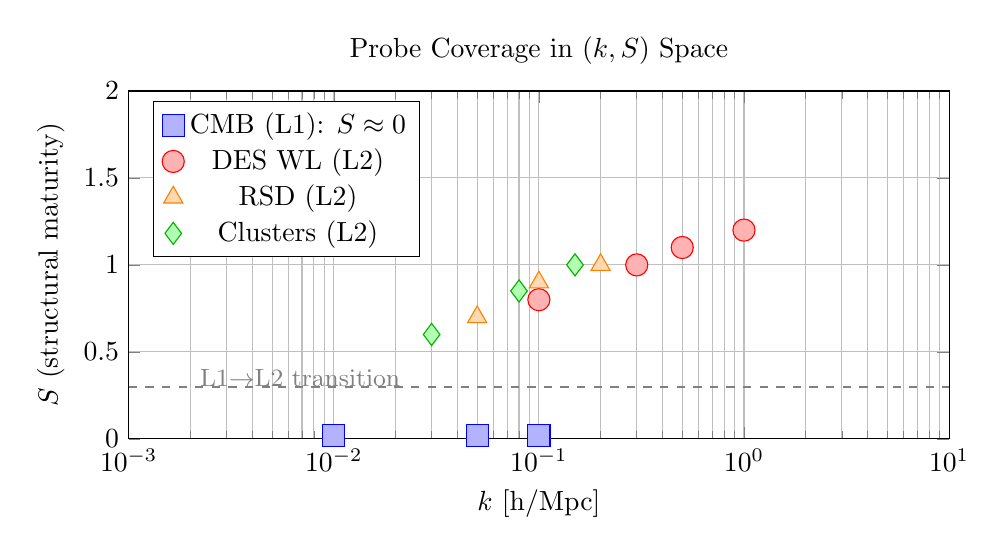
\begin{tikzpicture}
\begin{axis}[
    width=12cm,
    height=6cm,
    xlabel={$k$ [h/Mpc]},
    ylabel={$S$ (structural maturity)},
    xmode=log,
    xmin=0.001,
    xmax=10,
    ymin=0,
    ymax=2,
    grid=both,
    title={Probe Coverage in $(k,S)$ Space},
    legend pos=north west,
]

% CMB region (L1)
\addplot[
    only marks,
    mark=square*,
    mark size=4pt,
    color=blue,
    fill=blue!30,
] coordinates {(0.01, 0.02) (0.05, 0.02) (0.1, 0.02)};
\addlegendentry{CMB (L1): $S \approx 0$}

% DES WL region
\addplot[
    only marks,
    mark=*,
    mark size=4pt,
    color=red,
    fill=red!30,
] coordinates {(0.1, 0.8) (0.3, 1.0) (0.5, 1.1) (1.0, 1.2)};
\addlegendentry{DES WL (L2)}

% RSD region
\addplot[
    only marks,
    mark=triangle*,
    mark size=4pt,
    color=orange,
    fill=orange!30,
] coordinates {(0.05, 0.7) (0.1, 0.9) (0.2, 1.0)};
\addlegendentry{RSD (L2)}

% Cluster region
\addplot[
    only marks,
    mark=diamond*,
    mark size=4pt,
    color=green!70!black,
    fill=green!30,
] coordinates {(0.03, 0.6) (0.08, 0.85) (0.15, 1.0)};
\addlegendentry{Clusters (L2)}

% Transition zone
\draw[dashed, thick, gray] (axis cs:0.001, 0.3) -- (axis cs:10, 0.3);
\node[gray, anchor=west] at (axis cs:0.002, 0.35) {\small L1$\to$L2 transition};

\end{axis}
\end{tikzpicture}

\caption{\textbf{Top:} The regime response surface $R(k,S)$ with illustrative parameters ($R_0=0.05$, $a=0.1$, $b=0.3$, $c=0.05$). Response increases with both $k$ and $S$. \textbf{Bottom:} Schematic probe coverage in $(k,S)$ space. CMB (L1) probes low-$S$ regime where $R\approx 0$. Late-universe probes (WL, RSD, clusters) sample higher-$S$ regime where $R>0$, but overlap significantly in $(k,S)$ space, explaining their internal consistency. The L1$\to$L2 transition (dashed line) marks where gravitational response activates.}
\label{fig:response}
\end{figure}

\section{Falsification Protocol}

\subsection{Test 1: Tomographic Consistency}

DES Y6 provides tomographic bins across redshift. \textbf{All bins must follow a single global $R(k,S)$} with fixed $(R_0, a, b, c)$.

\textit{Failure criterion}: Fitting requires different parameters per bin.

\subsection{Test 2: Trend Sign Matching}

When two probes are matched to the same $k$-window AND the same $S/z$-window, they must show the same trend sign in any residuals from $\Lambda$CDM.

\textit{Failure criterion}: Probes with overlapping $(k,S)$ coverage show opposite deviations.

\subsection{Test 3: Predicted $S$-Gradient}

Given $R(k,S)$, compute the predicted $S_8$ offset as a function of effective redshift:
\begin{equation}
\Delta S_8(z_{\mathrm{eff}}) \propto R(k_{\mathrm{eff}}, S(z_{\mathrm{eff}}))
\end{equation}

This predicted gradient must be consistent with observed redshift trends in tomographic analyses.

\textit{Failure criterion}: Predicted gradient disagrees with observed redshift evolution.

\section{Epistemic Status}

\begin{table}[h]
\centering
\begin{tabular}{ll}
\toprule
\textbf{Component} & \textbf{Status} \\
\midrule
Regime-dependent $\mu$ & \checkmark\ Supported (Fugaku--DESI) \\
$\mu(k,z)$ formalism & \checkmark\ Supported (Weak Lensing paper) \\
$S$ as structural state & $\triangle$\ New, physically motivated extension \\
$R(k,S)$ response surface & $\triangle$\ New model structure \\
$k\times S$ interaction & $\triangle$\ Hypothesis, requires testing \\
L1$\leftrightarrow$L2 as primary tension locus & \checkmark\ Supported by DES Y6 internal consistency \\
\bottomrule
\end{tabular}
\end{table}

This framework does not claim validation. It provides the \textbf{minimal theoretical infrastructure} required to test whether EFC can explain structure growth phenomenology.

\section{Conclusion}

The $R(k,S)$ framework unifies prior EFC phenomenology into a single response surface:

\begin{enumerate}
    \item $\mu(a)$ from Fugaku--DESI $\to$ absorbed into $S$-dependence
    \item $\mu(k,z)$ from Weak Lensing $\to$ absorbed into $k$-dependence
    \item \textbf{New}: $S$ as state variable, making response physically grounded
\end{enumerate}

The key prediction is that the $S_8$ tension reflects an \textbf{L1$\to$L2 regime transition}, not systematic errors or probe-dependent physics. A single $R(k,S)$ surface should explain:
\begin{itemize}
    \item $\mu \approx 1$ at CMB ($S \approx 0$)
    \item $\mu > 1$ at late times ($S > 0$)
    \item Internal consistency within L2 (probes sample similar $S$ values)
\end{itemize}

This is testable with current data. Failure of the tomographic consistency test or the $S$-gradient prediction would falsify this formulation of EFC structure response.

\begin{thebibliography}{9}

\bibitem{fugaku}
Magnusson, M. (2026). ``Regime-Dependent Growth Enhancement: A Transition Metric Interpretation of the Fugaku--DESI Matter Density Offset.'' Figshare. \href{https://doi.org/10.6084/m9.figshare.31144030.v1}{doi:10.6084/m9.figshare.31144030.v1}

\bibitem{weaklens}
Magnusson, M. (2026). ``EFC Weak Lensing Phenomenology.'' Figshare. \href{https://doi.org/10.6084/m9.figshare.31188193.v1}{doi:10.6084/m9.figshare.31188193.v1}

\bibitem{desy6}
DES Collaboration (2026). ``Dark Energy Survey Year 6 Results: Cosmological Constraints from the Analysis of Cosmic Shear, Galaxy--Galaxy Lensing, and Galaxy Clustering.'' arXiv:2601.14559

\bibitem{planck}
Planck Collaboration (2020). ``Planck 2018 results. VI. Cosmological parameters.'' A\&A 641, A6.

\end{thebibliography}

\appendix

\section{Relation to Standard MG Parametrization}

In the standard modified gravity literature, perturbations are characterized by:
\begin{align}
k^2 \Psi &= -4\pi G a^2 \mu(k,a)\,\bar{\rho}\,\delta \\
\frac{\Phi}{\Psi} &= \gamma(k,a)
\end{align}

The $R(k,S)$ framework sets:
\begin{align}
\mu(k,a) &= 1 + R(k, S(a)) \\
\gamma(k,a) &= 1 \quad \text{(no gravitational slip in minimal EFC)}
\end{align}

\textbf{Note on $\gamma$}: The choice $\gamma = 1$ is a simplifying assumption in this minimal framework, not a fundamental requirement. Future extensions may allow $\gamma \neq 1$ to capture additional degrees of freedom. The present framework is modular: $R(k,S)$ can be constrained independently before relaxing the slip assumption.

This is directly implementable in CLASS/CAMB with appropriate modifications.

\section{Computing $S$ from Observables}

For a given background cosmology:
\begin{enumerate}
    \item Compute linear growth factor $D_{\mathrm{lin}}(z)$ from perturbation equations
    \item Compute nonlinear growth from halofit or N-body calibration
    \item $S(z) = \ln[\sigma_8^2(z) / \sigma_{8,\mathrm{lin}}^2(z)]$
\end{enumerate}

For DES Y6 tomographic bins:
\begin{itemize}
    \item Each bin has effective redshift $z_{\mathrm{eff}}$
    \item Compute $S(z_{\mathrm{eff}})$ for each bin
    \item This provides $\sim$10 points along the $S$-axis without free parameters
\end{itemize}

\vfill
\noindent\rule{\textwidth}{0.4pt}
\small Document version: 1.0 | 30 January 2026

\end{document}
